\documentclass[aspectratio=169, 10pt]{beamer}

\usepackage{bm} % bold math
\usepackage{fontspec}
\usepackage{minted}
\usepackage{pgf-pie}
\usepackage{tikz}

% Custom commands and environments
\makeatletter
\newcommand\version[1]{\renewcommand\@version{#1}}
\newcommand\@version{}
\def\insertversion{\@version}

\newcommand\course[1]{\renewcommand\@course{#1}}
\newcommand\@course{}
\def\insertcourse{\@course}

\newcommand\coursetitle[1]{\renewcommand\@coursetitle{#1}}
\newcommand\@coursetitle{}
\def\insertcoursetitle{\@coursetitle}

\newcommand\lecturenumber[1]{\renewcommand\@lecturenumber{#1}}
\newcommand\@lecturenumber{}
\def\insertlecturenumber{\@lecturenumber}
\makeatother

\newcommand{\slidetitle}[1]{{\xbseries \large \structure{#1}} \bigskip}
\newcommand{\term}[1]{{\color{blue} #1}}
\newcommand{\leftspace}{\hspace{1em}}
\newcommand{\inlinearrow}{
  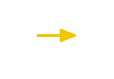
\begin{tikzpicture}[baseline]
    \node [anchor=base] (x) {};
    \draw [rawarrow] (x.mid west) -- ($(x.mid west) + (2em,0)$);
  \end{tikzpicture}
}

\newenvironment{slide}
{\begin{frame}[fragile,environment=slide]\vskip0pt plus 1filll}
{\vskip0pt plus 1filll\end{frame}}

% LaTeX

\setlength{\leftmargini}{1em}

% Common Information

\author{Jon Eyolfson}
\course{ECE 353}
\coursetitle{Systems Software}
\date{2024 Winter}

% fontspec

\defaultfontfeatures{Ligatures=TeX}
% \setmainfont{Domine}
\setsansfont{Inter}[
  FontFace={ul}{n}{Font=*-Thin},
  FontFace={el}{n}{Font=*-ExtraLight},
  FontFace={l}{n}{Font=*-Light},
  FontFace={sb}{n}{Font=*-SemiBold},
  FontFace={eb}{n}{Font=*-ExtraBold},
  FontFace={xb}{n}{Font=*-Black},
]
\setmonofont[Contextuals=AlternateOff, Ligatures=TeXOff]{Iosevka}[
  FontFace={xb}{n}{Font=*-Heavy},
]

%% Font Weights

\DeclareRobustCommand{\ulseries}{\fontseries{ul}\selectfont}
\DeclareTextFontCommand{\textul}{\ulseries}
\DeclareRobustCommand{\elseries}{\fontseries{el}\selectfont}
\DeclareTextFontCommand{\textel}{\elseries}
\DeclareRobustCommand{\lseries}{\fontseries{l}\selectfont}
\DeclareTextFontCommand{\textl}{\lseries}
\DeclareRobustCommand{\sbseries}{\fontseries{sb}\selectfont}
\DeclareTextFontCommand{\textsb}{\sbseries}
\DeclareRobustCommand{\ebseries}{\fontseries{eb}\selectfont}
\DeclareTextFontCommand{\texteb}{\ebseries}
\DeclareRobustCommand{\xbseries}{\fontseries{xb}\selectfont}
\DeclareTextFontCommand{\textxb}{\xbseries}

% tikz

\usetikzlibrary{
  arrows,
  arrows.meta,
  automata,
  backgrounds,
  calc,
  decorations.pathreplacing,
  matrix,
  positioning,
  overlay-beamer-styles,
  shapes,
  shapes.multipart,
  tikzmark,
}

\tikzstyle{rawarrow} = [
  -{Latex[round]},
  line width=1pt,
  yellow,
  shorten >=3pt,
  shorten <=3pt,
  font=\small,
  text=black,
]

\tikzstyle{arrow} = [
  -{Latex[round]},
  line width=1pt,
  yellow,
  shorten >=3pt,
  shorten <=3pt,
  transform canvas={yshift=3pt},
  font=\small,
  text=black,
]

\newcommand{\tikzmarkcoord}[1]{([yshift=3pt]pic cs:#1)}

% minted

\setminted{style=eyolfson, fontsize=\small, escapeinside=||}
\setmintedinline{fontsize=\normalsize}

% hyperref

\hypersetup{colorlinks, urlcolor=blue}

% beamer
\setbeamersize{text margin left=16mm, text margin right=16mm}
\setbeamertemplate{itemize items}[circle]
\setbeamercolor{item}{fg=black}
\setbeamercolor{structure}{fg=darkblue}
\setbeamerfont{frametitle}{series=\bfseries, parent=structure}
\setbeamertemplate{navigation symbols}{}
\setbeamertemplate{headline}{}
\setbeamertemplate{footline}{
  \begin{tikzpicture}[
    remember picture,
    overlay,
    shift={(current page.south west)},
  ]
    \path [fill=gray] (144mm, 0) -- (160mm, 16mm) -- (160mm, 0);
    \node [inner sep=3.5mm, outer sep=0, text=black, anchor=base east,
           align=right, yshift=3.5mm]
          at (current page.south east) {\ttfamily \small \insertframenumber{}};
  \end{tikzpicture}
}
\setbeamertemplate{title page}{
  \begin{tikzpicture}[
    remember picture,
    overlay,
    shift={(current page.south west)},
    background rectangle/.style={fill=darkblue},
    show background rectangle,
  ]
    \node [anchor=center, align=center, text=white, text width=40mm, scale=3.2]
          at (\paperwidth / 2, \paperheight * 2 / 3)
          {\xbseries \inserttitle{}};
    \node [anchor=base west, align=left, inner sep=0, text=white, yshift=2.5mm]
          at (16mm, \paperheight / 3)
          {\insertdate{} \insertcourse{}: \insertcoursetitle{}};
    \node [anchor=base west, align=left, inner sep=0, text=white, yshift=-2.5mm]
          at (16mm, \paperheight / 3)
          {\insertauthor};
    \node [anchor=base east, align=right, inner sep=0, text=white, yshift=2.5mm]
          at (144mm, \paperheight / 3)
          {Lecture \insertlecturenumber{}};
    \node [anchor=base east, align=right, inner sep=0, text=white,
           yshift=-2.5mm]
          at (144mm, \paperheight / 3)
          {\ttfamily \insertversion{}};
    \node [align=center, anchor=south, inner sep=0, text=white, yshift=3.5mm]
          (license) at (\paperwidth / 2, 0)
          {\fontsize{7pt}{7pt}\selectfont This  work is licensed under a
           \href{http://creativecommons.org/licenses/by-sa/4.0/}
                {\color{lightblue} Creative Commons Attribution-ShareAlike 4.0
                 International License}};
  \end{tikzpicture}
}

% xcolor

%% Primary Colour

\definecolor{pantone655}{RGB}{0, 42, 92} % #002a5c
\colorlet{darkblue}{pantone655}

%% Secondary Colours

\definecolor{pantone633}{RGB}{0, 139, 176} % #008bb0
\colorlet{blue}{pantone633}

\definecolor{pantonewarmred}{RGB}{220, 70, 51} % #dc4633
\colorlet{red}{pantonewarmred}

\definecolor{pantone3285}{RGB}{0, 161, 137} % #00a189
\colorlet{cyan}{pantone3285}

\definecolor{pantone7722}{RGB}{13, 83, 77} % #0d534d
\colorlet{darkcyan}{pantone7722}

\definecolor{pantone376}{RGB}{141, 191, 46} % #8dbf2e
\colorlet{green}{pantone376}

\definecolor{pantone2613}{RGB}{109, 36, 122} % #6d247a
\colorlet{violet}{pantone2613}

\definecolor{pantone2985}{RGB}{111, 199, 234} % #6fc7ea
\colorlet{lightblue}{pantone2985}

\definecolor{pantone227}{RGB}{171, 19, 104} % #ab1368
\colorlet{magenta}{pantone227}

\definecolor{pantone7406}{RGB}{241, 197, 0} % #f1c500
\colorlet{yellow}{pantone7406}

%% Neutrals

\definecolor{pantonecoolgray2}{RGB}{208, 209, 201} % #d0d1c9
\colorlet{gray}{pantonecoolgray2}


\lecturenumber{24}
\title{Locking}
\version{2.0.0}

\begin{document}

  \begin{frame}[plain, noframenumbering]
    \titlepage
  \end{frame}

  \begin{slide}
    \slidetitle{Monitors Are Built Into Some Languages}

    With object-oriented programming, developers wanted better ease of use
    \medskip

    Could mark a method as monitored, and let the compiler handle locking

    \leftspace{}An object can only have one thread active in its monitored
    methods
    \medskip

    It's basically one mutex per object, created for you

    \leftspace{}The compiler inserts calls to lock and unlock

  \end{slide}

  \begin{slide}

    \slidetitle{Java's \texttt{synchronized} Keyword is an Example of a Monitor}

    \begin{minted}{c}
public class Account {
  int balance;
  public synchronized void deposit(int amount)  { balance += amount; }
  public synchronized void withdraw(int amount) { balance -= amount; }
}
    \end{minted}
    \medskip

    the compiler transforms to:
    \medskip

    \begin{minted}{c}
public void deposit(int amount) {
  lock(this.monitor); /* New */
  balance += amount;
  unlock(this.monitor); /* New */
}
public void withdraw(int amount) {
  lock(this.monitor); /* New */
  balance -= amount;
  unlock(this.monitor); /* New */
}
    \end{minted}
  \end{slide}

  \begin{slide}

    \slidetitle{Condition Variables Behave Like Semaphores}

    You can create your own custom queue of threads
    \medskip

    \begin{minted}{c}
#include <pthread.h>

int pthread_cond_init(pthread_cond_t *cond,
                      const pthread_condattr_t *attr)
int pthread_cond_destroy(pthread_cond_t *cond);
int pthread_cond_signal(pthread_cond_t *cond);
int pthread_cond_broadcast(pthread_cond_t *cond);
int pthread_cond_wait(pthread_cond_t *cond, pthread_mutex_t *mutex);
int pthread_cond_timedwait(pthread_cond_t *cond, pthread_mutex_t *mutex,
                           const struct timespec *abstime);
    \end{minted}
    \medskip

    The \texttt{wait} functions add this thread to the queue

    \leftspace{}\texttt{signal} wakes up one thread, \texttt{broadcast} wakes
    up all threads

  \end{slide}

  \begin{slide}

    \slidetitle{Condition Variables MUST Be Paired with a Mutex}

    Any calls to \texttt{wait} must already hold the mutex

    \leftspace{}(\texttt{signal} and \texttt{broadcast} may not)
    \medskip

    Why? Think that \texttt{wait} needs to add itself to the queue safely (no
    data races)

    \leftspace{}It needs the mutex as an argument to unlock it before going to
    sleep

    \leftspace{}\leftspace{}The thread will hold the locked \texttt{mutex}
    before and after
    the call
    \medskip

    One mutex can also protect multiple condition variables
    \medskip

    We'll only consider calls to \texttt{wait} and \texttt{signal}

  \end{slide}

  \begin{slide}

    \slidetitle{The \texttt{wait} Call Does Not Contain Data Races}

    Understand what \texttt{wait} does (for condition variables!)
    \medskip

    The thread calling \texttt{wait}:

    \begin{enumerate}
      \item Adds itself to the queue for the condition variable
      \item Unlock the mutex
      \item Gets blocked (it can no longer be scheduled to run)
    \end{enumerate}
    \medskip

    The thread calling \texttt{wait} needs another thread to call \texttt{signal} or
    \texttt{broadcast},

    then if it's selected:

    \begin{enumerate}
      \item Gets unblocked (it can be scheduled to run)
      \item Tries to lock the mutex again, \texttt{wait} returns when it gets it
    \end{enumerate}

  \end{slide}

  \begin{slide}

    \slidetitle{We Can Use Condition Variables for Our Producer/Consumer}

    \begin{columns}
      \begin{column}{0.5\textwidth}
        \begin{minted}{c}
pthread_mutex_t mutex;
int nfilled;
pthread_cond_t has_filled;
pthread_cond_t has_empty;

void producer() {
  // produce data
  pthread_mutex_lock(&mutex);
  while (nfilled == N) {
    pthread_cond_wait(&has_empty,
                      &mutex);
  }
  // fill a slot
  ++nfilled;
  pthread_cond_signal(&has_filled);
  pthread_mutex_unlock(&mutex);
}
        \end{minted}
      \end{column}
      \begin{column}{0.5\textwidth}
        \begin{minted}{c}
void consumer() {
  pthread_mutex_lock(&mutex);
  while (nfilled == 0) {
    pthread_cond_wait(&has_filled,
                      &mutex);
  }
  // empty a slot
  --nfilled;
  pthread_cond_signal(&has_empty);
  pthread_mutex_unlock(&mutex);
  // consume data
}
        \end{minted}
      \end{column}
    \end{columns}

  \end{slide}

  \begin{slide}

    \slidetitle{What's the Issue with the Following Code?}

    \begin{minted}{c}
/* Thread 1 */
pthread_mutex_lock(&mutex);
while (!condition) {
  pthread_cond_wait(&cond, &mutex);
}
pthread_mutex_unlock(&mutex);

/* Thread 2 */
condition = true;
pthread_cond_signal(&cond);
    \end{minted}

  \end{slide}

  \begin{slide}

    \slidetitle{Can We Change the \texttt{while} to an \texttt{if}?}

    \begin{minted}{c}
/* Thread 1 */
pthread_mutex_lock(&mutex);
if (!condition) {
  pthread_cond_wait(&cond, &mutex);
}
// What could happen here?
pthread_mutex_unlock(&mutex);

/* Thread 2 */
pthread_mutex_lock(&mutex);
condition = true;
pthread_mutex_unlock(&mutex);
pthread_cond_signal(&cond);

/* Thread 3 */
pthread_mutex_lock(&mutex);
condition = false;
pthread_mutex_unlock(&mutex);
    \end{minted}

  \end{slide}

  \begin{slide}

    \slidetitle{Condition Variables Serve a Similar Purpose as Semaphores}

    You can think of semaphores as a special case of condition variables

    \leftspace{}They go to sleep when the value is 0, when it's greater
    than 0 they wake up
    \medskip

    You can implement one using the other, however it can get messy
    \medskip

    For complex conditions condition variables offer much better clarity

  \end{slide}

  \begin{slide}

    \slidetitle{Locking Granularity is the Extent of Your Locks}

    You need locks to prevent data races
    \medskip

    Lock large sections of your program, or divide the locks and
    use smaller sections?

    \leftspace{}What if you want to parallelize your hash table?
    \medskip
    
    Things to consider about locks:
    \begin{itemize}
     \item Overhead
      \item Contention
      \item Deadlocks
    \end{itemize}

  \end{slide}

  \begin{slide}

    \slidetitle{Locking Overheads}

    \begin{itemize}
      \item Memory allocated
      \item Initialization and destruction time
      \item Time to acquire and release locks
    \end{itemize}

    The more locks you have, the greater each cost is going to be

  \end{slide}

  \begin{slide}

    \slidetitle{You Do NOT Want Deadlocks}

    The more locks you have, the more you have to worry about deadlocks
    \medskip

    Conditions for deadlocking:

    \begin{enumerate}
      \item Mutual Exclusion (of course for simple locks)
      \item Hold and Wait (you have a lock and try to acquire another)
      \item No Preemption (we can't take simple locks away)
      \item Circular Wait (waiting for a lock held by another process)
    \end{enumerate}

  \end{slide}

  \begin{slide}

    \slidetitle{A Simple Deadlock Example}

    Consider two processors trying to get two {\it locks}:
    \medskip

    \begin{columns}
      \column{0.4\textwidth}
        {\bf Thread 1}

        \verb+Get Lock 1+

        \verb+Get Lock 2+

        \verb+Release Lock 2+

        \verb+Release Lock 1+
      \column{0.4\textwidth}
        {\bf Thread 2}

        \verb+Get Lock 2+

        \verb+Get Lock 1+

        \verb+Release Lock 1+

        \verb+Release Lock 2+
    \end{columns}
    \medskip

    T11 gets Lock 1, then T2 gets Lock 2, now
    they both wait for each other

    \leftspace{}Deadlock

  \end{slide}

  \begin{slide}

    \slidetitle{You Can Ensure Order to Prevent Deadlocks}

    \begin{minted}{c}
void f1() {
    locktype_lock(&l1);
    locktype_lock(&l2);
    // protected code
    locktype_unlock(&l2);
    locktype_unlock(&ll);    
}
    \end{minted}
    \medskip

    This code will not deadlock, you can only get {\tt l2} if you have
    {\tt l1}

  \end{slide}

  \begin{slide}

    \slidetitle{You Could Also Prevent A Deadlock by Using {\tt trylock}}

    Remember, for {\tt pthread} there's {\tt trylock} that returns 0 if it gets
    the lock
    \medskip

    \begin{minted}{c}
void f2() {
    locktype_lock(&l1);
    while (locktype_trylock(&l2) != 0) {
        locktype_unlock(&l1);
        // wait
        locktype_lock(&l1);
    }
    // protected code
    locktype_unlock(&l2);
    locktype_unlock(&ll);    
}
    \end{minted}
    \medskip

    This code will not deadlock, it will give up {\tt l1} if it can't get
    {\tt l2}

  \end{slide}

  \begin{slide}

    \slidetitle{We Explored More Advanced Locking}

    We have another tool to ensure order

    \begin{itemize}
      \item Condition variables are clearer for complex condition signaling
      \item Locking granularity matters
      \item You must prevent deadlocks
    \end{itemize}

  \end{slide}

\end{document}
